%% The following is a directive for TeXShop to indicate the main file
%%!TEX root = diss.tex

\chapter{Introduction}
\label{ch:Introduction}
Haptic sensations enable engaging, personal, and low-attention experiences, but this is limited due to little support for \emph{designing} a haptic sensation.
Computer-controlled haptic experiences are a recent phenomenon; the focus on technology requirements and rapidly changing field has left little room for examining processes of design in a methodical way.
In this dissertation, I propose to study the process of haptic experience design (``HaXD") to understand how to build interactive software to support haptic experience designers.

While many tools exist to support design in other modalities, such as graphic design, there are few for haptics.
Part of this comes from immaturity of the field and lack of market penetration of highly expressive haptic devices.
However, there are also intrinsic challenges to designing for the sense of touch.
I want to develop practical tools that support the HaXD process, building a body of knowledge of how to facillitate this difficult subfield of design.
I approach this problem with two different strategies:
\begin{enumerate}
\item \textbf{Vibrotactile design case studies.}
To understand design, I take a design perspective.
In each of three case studies, I design, build, and evaluate a tool to support an aspect of haptic experience design, scoped to \emph{vibrotactile} (VT) design.
Each of these results in concrete implications for designing tools and a small window onto the larger HaXD process.
Contributions include algorithms, data structures, interaction techniques, features, and working software tools that have been employed by designers.
\autoref{ch:hapticinstrument}, \autoref{ch:hapticanimation}, and \autoref{ch:hapticexamples} outline these.

\item \textbf{Synthesis into preliminary theory.}
While the case studies provide an in-depth investigation into vibrotactile sensation design, results may not generalize to other devices.
Furthermore, despite the recent growth of the field, haptic designers remain relatively rare and difficult to recruit.
To generalize our findings to other situations and ground it with haptic experience designers, I plan to draw from other data sources: a workshop held at World Haptics 2015, already-collected interviews with haptic designers, and a number of side-projects.
This synthesized contribution will help refine our findings, such as tasks, goals, barriers, strategies, and practices designers use and face when working with haptics.
\end{enumerate}


\begin{figure}[htbp]
\begin{center}
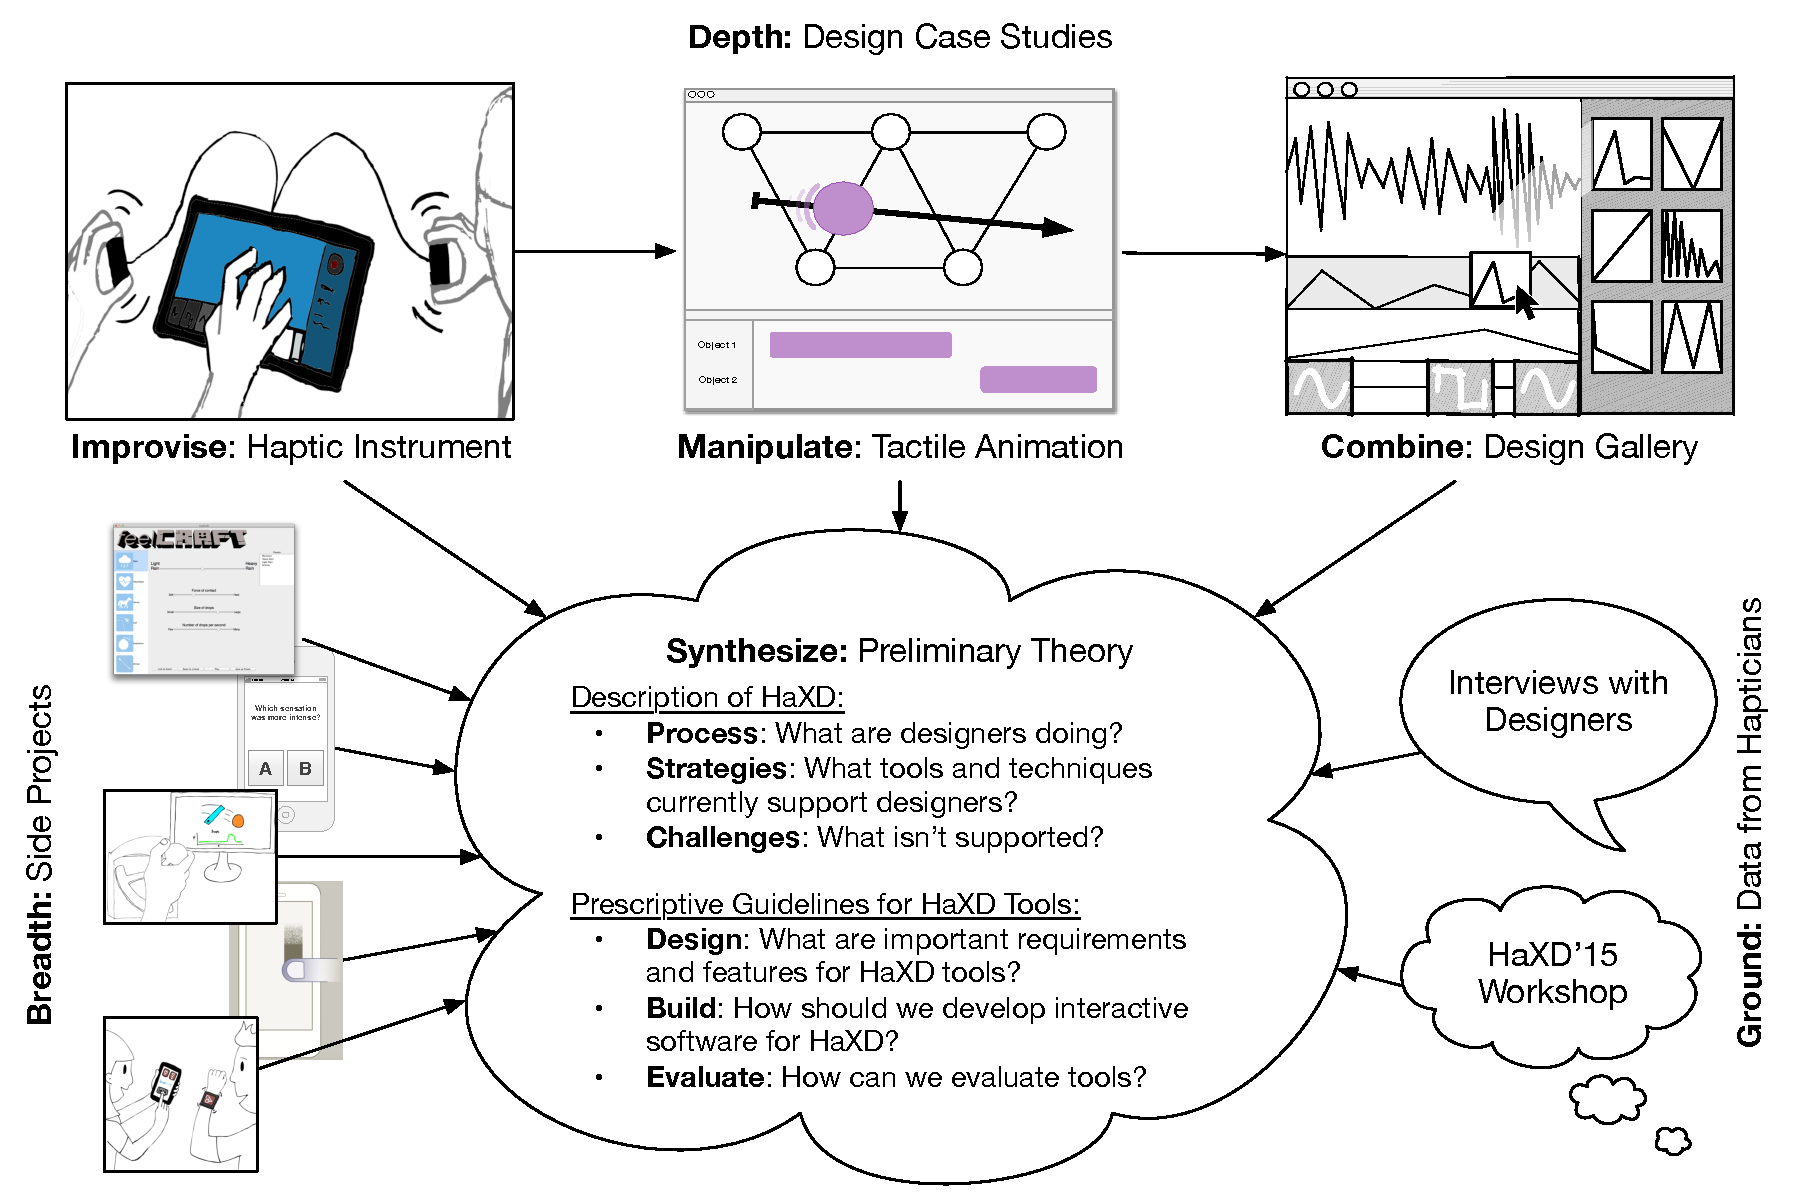
\includegraphics[width=\textwidth]{HaXDTheoryOutline-2015-05-22}
\caption{Methodology overview. Three case studies investigate VT tools in-depth; findings are synthesized with side projects and grounded data into a preliminary theory.}
\label{fig:intro:methodologyoverview}
\end{center}
\end{figure}


\section{Vibrotactile Design Case Studies}

Each case study investigates a different set of design concepts with varying user populations, VT device, and design challenges (\autoref{fig:intro:casestudyoverview}), but restricts scope to VT sensations.
This offers a deep look into an expressive and increasingly common class of haptic devices, allowing us to explore critical features in a somewhat controlled fashion.
An iterative approach allows us to refine ideas and methods, and so each case study follows three steps: \emph{gather}, finding requirements and previous design elements; \emph{create}, where we design and build the tool; and \emph{evaluate}, where we test the tool with its target population and consolidate lessons learned.

In Study 1, the Haptic Instrument, we focus on real-time, rapid design of VT sensations with a first look into themes of real-time design and collaboration.
When participants worked with our tool, mHIVE (a ``mobile Haptic Instrument for Vibrotactile Exploration"), compositions couldn't be edited, suggesting mHIVE was suitable for exploration and improvised communication, but not as suited to refining ideas.
This informed Study 2, Tactile Animation, where we developed a single abstracted animation object directly manipulated in both space and time.
Animators found our tactile animation tool, Mango, easy-to-use, and confirmed our findings about the value of real-time exploration.


\begin{figure}[htbp]
\begin{center}
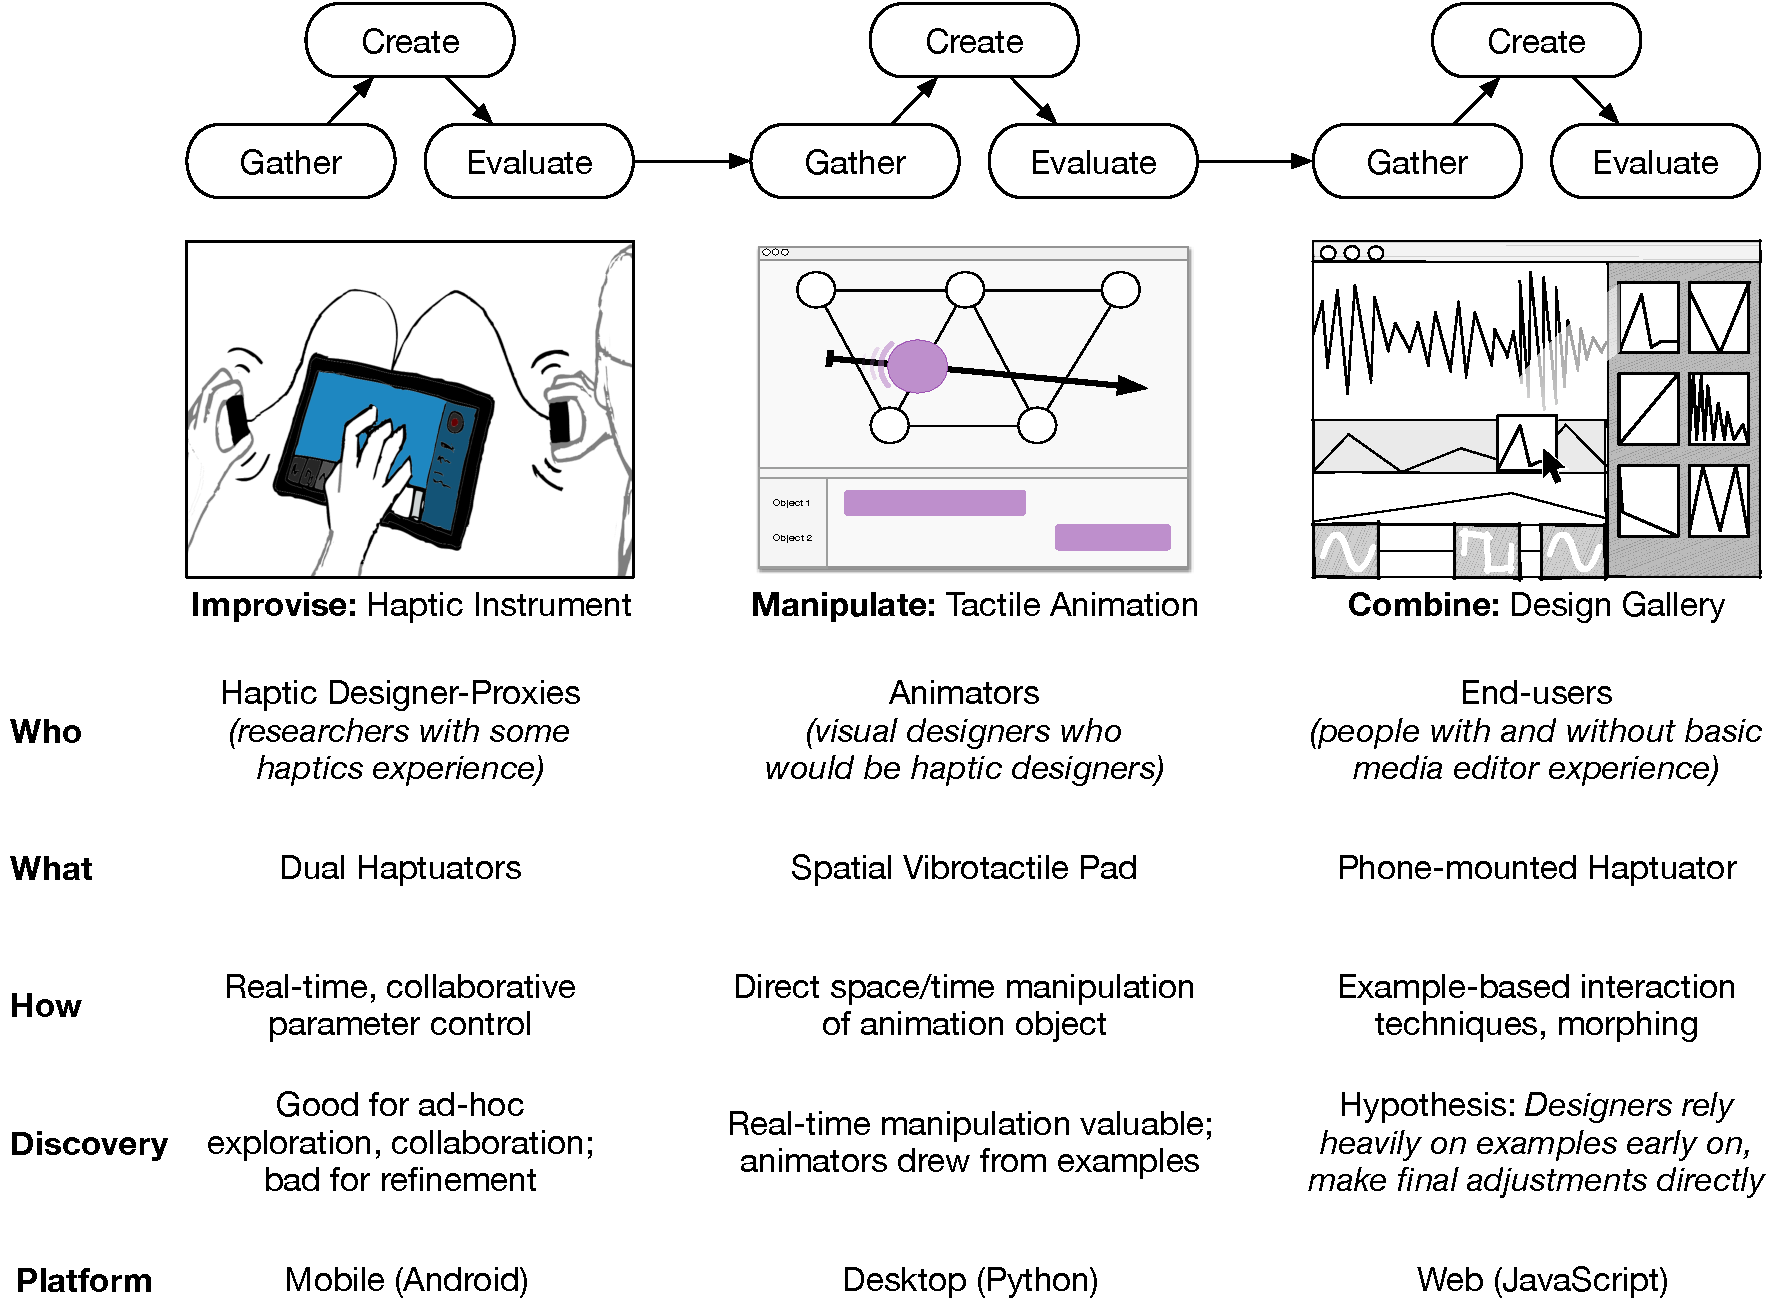
\includegraphics[width=\textwidth]{HaXDTheoryCaseStudyOutline-2015-05-28}
\caption{Vibrotactile design case studies. Each studies an aspect of vibrotactile design with a varied set of users, devices, platforms, and foci.}
\label{fig:intro:casestudyoverview}
\end{center}
\end{figure}

One stand-out result from both Mango and mHIVE is that designers drew from their experience or examples found in the world, and wanted to re-use what they had created (e.g., through copy and paste).
In Study 3, I explore the role of examples in haptic design.
This study is codenamed ``Project Macaron" and consists of two phases.
Phase I, ``algorithms and interaction techniques", builds a set of perceptually-verified ways to manipulate examples and incorporate them into designs.
In Phase II, we use the results of Phase I to create a haptic design gallery interface, and study how and when users incorporate examples into their VT designs.
In this way we hope to consolidate our findings from mHIVE and Mango, and capture our participants' design process more concretely through logging of user actions.

These studies are described in more detail in \autoref{ch:hapticinstrument},  \autoref{ch:hapticanimation}, and \autoref{ch:hapticexamples}.
Each chapter is presented as an outline of what will appear in the final dissertation, summarizing methods and results for completed work and outlining planned work.


\section{Synthesis of Contributions}

Each case study provides concrete knowledge for building a vibrotactile authoring tool, and some insight into the vibrotactile design process.
However, haptic technology consists of many devices and experiences beyond vibrotactile.
%In addition, it is difficult to find and recruit haptic designers.
I will synthesize findings from the three design case studies together with a number of side projects, the design literature, community feedback from a workshop on haptic experience design, and interviews with haptic designers into a preliminary design theory on how to support the creation of engaging, captivating haptic experiences.
I expect to make progress on the following questions:
\begin{enumerate}
    \item \textbf{Description of the Haptic Design Process.}
    What are the major \textbf{processes and tasks} conducted by haptic designers?
    What \textbf{strategies} do haptic designers employ, including existing tools?
    What are the \textbf{challenges} haptic designers face?
    
    
    \item \textbf{Prescriptive Implications for HaXD Tools.}
    What are major \textbf{requirements} and \textbf{features} for designing HaXD tools?
    What are some considerations when \textbf{implementing} HaXD tools in software?
    How can we \textbf{evaluate} design tools effectively?
\end{enumerate}

This process is described in \autoref{ch:haxd}.


\section{Summary of Progress}

I am currently working on the \emph{create} stage of the third case study; the first two have papers either published or in peer-review.
Multiple side projects are underway, primarily  carried out by undergraduate students I'm co-supervising.
All side projects are expected to be substantially developed or completed by the end of summer 2015; the FeelCraft side project has already been published and presented.
For more information on current progress, please see \autoref{ch:timeline}.


The proposal continues as follows.
First, in \autoref{ch:rw}, I cover related work with an overview of haptic technology and applications, a presentation of existing haptic design tools, and a discussion of design theory from other fields.
Then, I outline each VT design case study in \autoref{ch:hapticinstrument},  \autoref{ch:hapticanimation}, and \autoref{ch:hapticexamples}.
%Each chapter is presented as a direct outline of what will appear in the final dissertation, summarizing either methods and results (\autoref{ch:hapticinstrument} and \autoref{ch:hapticanimation}) or proposed methods and possible results (\autoref{ch:hapticexamples}).
After, I describe the planned data synthesis in more detail in \autoref{ch:haxd}.
Finally, I present milestones and a timeline for my PhD in \autoref{ch:timeline}.


%
% END
%
\endinput

Any text after an \endinput is ignored.
You could put scraps here or things in progress.
